To successfully solve a RoboCup@Home challenge, a robot needs a basic understanding of the environment: it needs to know how to get from A to B without colliding, it must be able to detect humans and objects with which it has to interact and it must localize itself with respect to the objects it has to manipulate.
Therefore, \gls{ed}, a 3D, object-based, volumetric world model was developed.
The datastructures and algorithms used in this world model are described in the 2015 TDP.
More information and tutorials can be found on our Github page\footnote{\texttt{https://github.com/tue-robotics/ed}}.

\gls{ed} depends on having an accurate description of the world, including the locations of walls and furniture.
However, tables, chairs and even cabinets may move in a household environment.
If the world model is not updated accordingly, two important problems arise:
\begin{itemize}
    \item The robot will not position itself correctly with respect to the furniture (cabinet, table, etc) when it needs to interact with or inspect these entities
    \item Since \gls{ed} uses background subtraction for object segmentation, segmentation may not work correctly
\end{itemize}

\begin{figure}[ht]
        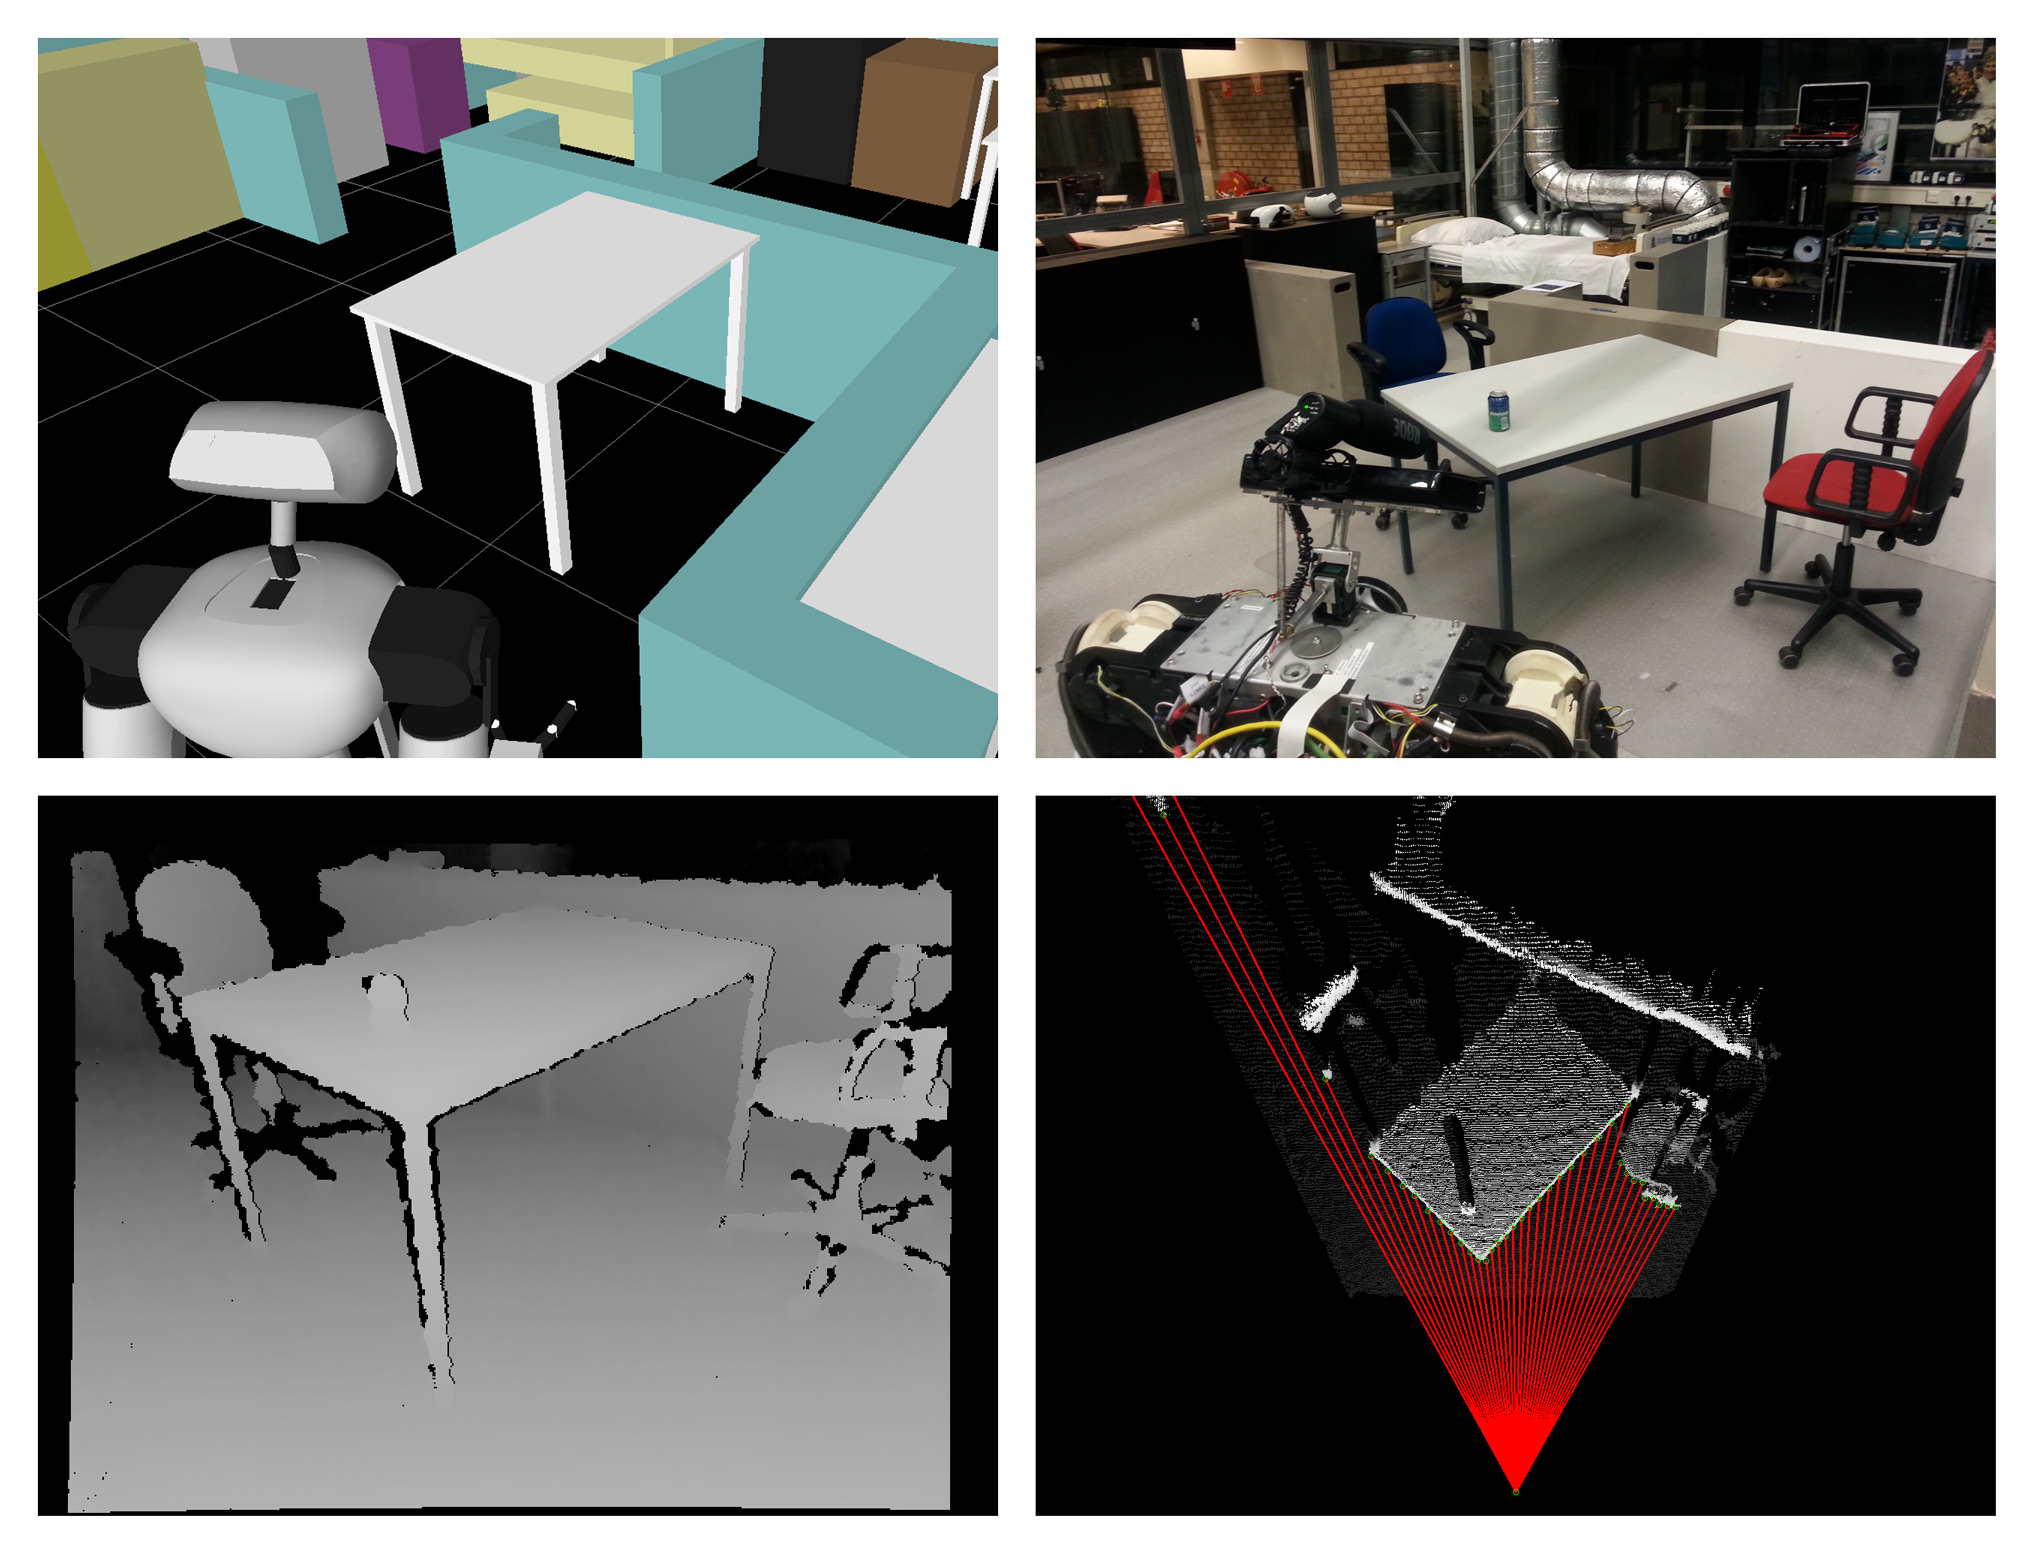
\includegraphics[width = \linewidth]{Figures/fitting-small}
        \caption{World model furniture fitting algorithm. Top-left: world model visualization as the robot thinks the world is. Top-right: actual situation: the table is rotated and moved. Bottom-left: depth image obtained from the depth sensor (brighter means closer). Bottom-right: top-down projected point cloud (brighter means closer); dividing the points into beams, 2D range data can be extracted and used for efficient template fitting.}
        \label{fig:fitting}
\end{figure}

To deal with this, and to get rid of pre-defined location definitions in general, an \gls{ed}-plugin was developed which can estimate the positions of furniture in the room.
This pose estimation algorithm works as follows (also see Figure~\ref{fig:fitting}):
\begin{enumerate}
    \item The camera pose with respect to the floor is obtained using the robot location and forward kinematics
    \item The point cloud obtained from the depth camera is transformed to the robot's base frame using the camera pose
    \item All points belonging to the floor are filtered using a simple height check per point. All other points are projected onto the floor (resulting in a top-down view).
    \item Then, all projected points are divided into beams that originate at the camera origin. The closest point per beam is stored. This results in a 1-dimensional array of ranges, very similar to the sensor data obtained from a laser range finder. However, the ranges obtained from this algorithm do not simply represent a planar cross-section of the world, but a projection of all points except the ground. This allows the data to also correctly represent a table (while a laser range finder would probably scan above or below the table top)
    \item A top-down 2D contour model is created from the 3D model that needs to be fitted into the sensor data
    \item A simple template-matching algorithm is used to fit the 2D contour model into the 1-dimension range data, resulting in the 2D-pose (x, y, yaw) of the model 
\end{enumerate}

The conversion from a 3D point cloud to a 1-dimension range array enables the use of a very efficient fitting algorithm, which allows for constant tracking of entities at high update rates. Do note, however, that the following assumptions are made:
\begin{itemize}
    \item The entity that needs to be fitted is standing on the ground, and is merely translated along the floor plane, and rotated along the vertical axis (only yaw, no roll or pitch)
    \item The entity is not occluded for large parts by other entities
    \item A 2D top-down contour model is available, or can be constructed from a 3D model
\end{itemize}

Fortunately, these assumptions hold in many situations when trying to estimate the poses of furniture. Several experiments in real situations have shown that the fitting strategy is indeed efficient and effective in many situations.